\documentclass[letter,11pt]{article}
\usepackage[utf8]{inputenc}

\usepackage[cm]{fullpage}
\usepackage{color}
\usepackage{hyperref}
\usepackage{mdwlist}

\hypersetup{breaklinks=true,%
pagecolor=white,%
colorlinks=true,%
linkcolor=cyan,%
urlcolor=MyDarkBlue}

\definecolor{MyDarkBlue}{rgb}{0,0.0,0.45}

%%%%%%%%%%%%%%%%%%%%%%%%%%
% Formatting parameters  %
%%%%%%%%%%%%%%%%%%%%%%%%%%

\newlength{\tabin}
\setlength{\tabin}{1em}
\newlength{\secsep}
\setlength{\secsep}{0.1cm}

\setlength{\parindent}{0in}
\setlength{\parskip}{0in}
\setlength{\itemsep}{0in}
\setlength{\topsep}{0in}
\setlength{\tabcolsep}{0in}

\definecolor{contactgray}{gray}{0.3}
\pagestyle{empty}

%%%%%%%%%%%%%%%%%%%%%%%%%%
%  Template Definitions  %
%%%%%%%%%%%%%%%%%%%%%%%%%%

\newcommand{\lineunder}{\vspace*{-8pt} \\ \hspace*{-6pt} \hrulefill \\ \vspace*{-15pt}}
\newcommand{\name}[1]{\begin{center}\textsc{\Huge#1}\\\end{center}}
\newcommand{\program}[1]{\begin{center}\textsc{#1}\end{center}}
\newcommand{\contact}[1]{\begin{center}\color{contactgray}{\small#1}\end{center}}

\newenvironment{tabbedsection}[1]{
  \begin{list}{}{
      \setlength{\itemsep}{0pt}
      \setlength{\labelsep}{0pt}
      \setlength{\labelwidth}{0pt}
      \setlength{\leftmargin}{\tabin}
      \setlength{\rightmargin}{\tabin}
      \setlength{\listparindent}{0pt}
      \setlength{\parsep}{0pt}
      \setlength{\parskip}{0pt}
      \setlength{\partopsep}{0pt}
      \setlength{\topsep}{#1}
    }
  \item[]
}{\end{list}}

\newenvironment{nospacetabbing}{
    \begin{tabbing}
}{\end{tabbing}\vspace{-1.2em}}

\newenvironment{resume_header}{}{\vspace{0pt}}


\newenvironment{resume_section}[1]{
  \filbreak
  \vspace{2\secsep}
  \textsc{\large#1}
  \lineunder
  \begin{tabbedsection}{\secsep}
}{\end{tabbedsection}}

\newenvironment{resume_subsection}[2][]{
  \textbf{#2} \hfill {\footnotesize #1} \hspace{2em}
  \begin{tabbedsection}{0.5\secsep}
}{\end{tabbedsection}}

\newenvironment{subitems}{
  \renewcommand{\labelitemi}{-}
  \begin{itemize}
      \setlength{\labelsep}{1em}
}{\end{itemize}}

\newenvironment{resume_employer}[4]{
  \vspace{\secsep}
  \textbf{#1} \\ 
  \indent {\small #2} \hfill {\footnotesize#3 (#4)}
  \begin{tabbedsection}{0pt}
  \begin{subitems}
}{\end{subitems}\end{tabbedsection}}

%====================
% OFFICIAL PUBLIC OVERLEAF TEMPLATE
% https://www.overleaf.com/latex/templates/data-science-tech-resume-template/zcdmpfxrzjhv
% 
%====================
%
% Resume template for data scientists, a complement to data-science-tech-cover-letter-template:
% https://www.overleaf.com/latex/templates/data-science-tech-cover-letter-template/gbrcqktbsfxf
%
% Files:        resume.tex: Main file
%               _header.tex: header code
%               TLCresume.sty: style file containing formatting details
%               section/objective: https://www.indeed.com/career-advice/resumes-cover-letters/resume-objective-examples
%               section/skills: table of skills
%               section/experience: projects or roles
%               section/education: schools and stuff
%               section/activities: optional, could comment out in resume.tex.
%
% Editor:       https://github.com/TimmyChan
%               https://www.linkedin.com/in/timmy-l-chan/
%               
% Last Updated: July 5 2022
%
%====================


\usepackage{TLCresume}

%====================
% CONTACT INFORMATION
%====================
\def\name{Maeva N'guessan} % Name Here
\def\phone{06.27.85.02.74}
\def\LinkedIn{LinkedIn : Maeva N'GUESSAN} % linkedin.com/in/______
\def\city{Evry-Courcouronnes }
\def\email{maevanguessan@outlook.fr}
\def\role{Stagiaire } % JOB TITLE 



%====================
%====================
% Header: Contact
%====================

\RequirePackage{fancyhdr}
\fancypagestyle{fancy}{%
\fancyhf{}


\lhead{\phone\vspace{.1em}\\ \\ % PHONE    
        \city\vspace{.1em}\\ \\ % city
        \LinkedIn\vspace{.1em}\\ \\
        \href{https://www.maevaportfolio.com}
       {www.maevaportfolio.com}\\ 
	    \href{mailto:\email}{\email}} % EMAIL}
	\chead{%
	    \centering {\Huge \skills \name \vspace{.3em}} \\ % feel free to adjust vspace to 0 
	    {\color{highlight} \Large{\role\vspace{.9em}\\}}} %
        
	    \rhead{
	    
     {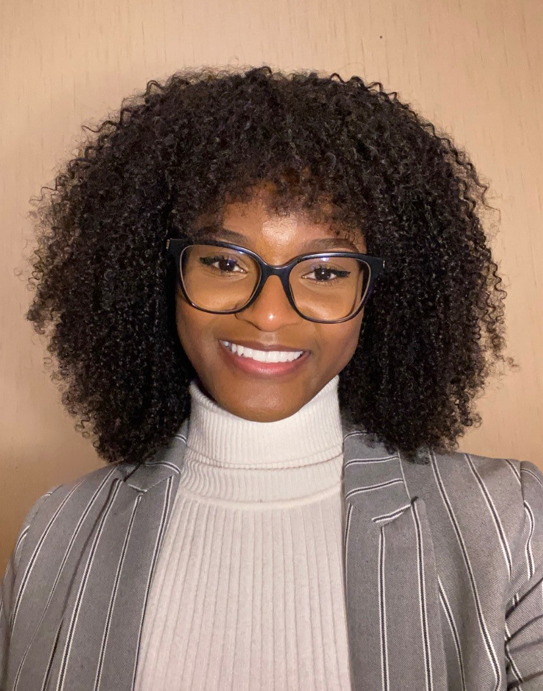
\includegraphics[width=30mm]{maphoto.png}}} % LinkedIn  
     \\

\renewcommand{\headrulewidth}{1pt}% 2pt header rule
\renewcommand{\headrule}{\hbox to\headwidth{%
  \color{highlight}\leaders\hrule height \headrulewidth\hfill}}
}
\pagestyle{fancy} 

\setlength{\headheight}{83pt}
\setlength{\headsep}{29pt}


\begin{document}
%====================
% Objective Statement
%====================
\subsection{}
Actuellement en master Économétrie et Statistiques à l’université Paris I Panthéon-Sorbonne, j’ai un fort attrait pour la data science et l’application de compétences informatiques à l’économie. Je souhaite développer mes connaissances en effectuant un stage d’une durée de 4 à 6 mois à partir de Février en temps partiel puis Avril en temps plein. 


\section{FORMATION}
\skills{Master 1 Économétrie, Statistiques}, \ \textit{Paris 1 Panthéon-Sorbonne, \ Paris} \hfill\textbf{Septembre 2023- Juillet 2024} 
\vspace{-10pt}
\begin{zitemize}
\item Machine Learning ( Xgboost, random forest), Économétrie pour la santé, séries temporelles et Microéconomie.
\item Informatique : Python, R, SAS, & SAS/IML.

\end{zitemize}
\skills{Licence d'Économie mineure Informatique}, \ \textit{Paris 1 Panthéon-Sorbonne, \ Paris} \hfill\textbf{mars 2021- juin 2023} 
\vspace{-10pt}
\begin{zitemize}
\item Économétrie, Mathématiques, Statistiques, Macroéconomie et Microéconomie.
\item Informatique : MySQL, Python, Excel VBA, R.
 
\end{zitemize}
\vspace{-2pt}
\skills{Classe préparatoire aux Grandes Écoles de Commerces}, \ \textit{Lycée Hoche, Versailles} \hfill\textbf{sept 2020- mars 2021}
\\

\section{EXPERIENCE} 
\skills {Chargée d'enquêtes statistiques}, \textit{BB Players (freelance)} \hfill\textbf{Janvier 2023}
\vspace{-5pt}
\begin{zitemize}
\item Mailing et récupération des données des clubs de basket sur internet. 
\item Analyse des résultats de l'enquête BB Players.
\item Rédaction de synthèse et création de Dashboard sur Excel.
\end{zitemize}


\vspace{-5pt}
\section{PROJETS PERSONNELS}


%====================
% EXPERIENCE D
%====================

\subsection{{PROJET PREDICTION DU RENDEMENT DES CULTURES\hfill  Août 2023 }}
\begin{zitemize}
\item Objectif : Faciliter la prévision du rendement des cultures agricoles selon plusieurs critères
\item Librairie utilisées : numpy, pandas, matplotlib, seaborn, scikit-learn, pickle pour le déploiement
\item Résultats : Développement d’une API en utilisant
Flask et HTM
\end{zitemize}


%====================
% EXPERIENCE A
%====================
\subsection{{PRÉVISION D'UN CRÉDIT LOGEMENT MACHINE LEARNING AVEC STREAMLIT \hfill Juillet 2022 }}
\begin{zitemize}
\item Objectif : Création d’un modèle machine learning afin de prédire l’attribution de prêt bancaire. 
\item  Librairies utilisées : pandas, numpy, matplotlib et seaborn. Création d'un model de régression logistique.
\item Résultats : Réalisation d'une application web interactive à l'aide de Streamlit. permettant d’enregistrer les données d’un client. 
\end{zitemize}



%====================
% EXPERIENCE B
%====================
\subsection{{PROJET R SHINY SUR LES ARRESTATIONS AUX ETATS-UNIS \hfill  Décembre 2022 }}
\begin{zitemize}
\item Objectif : Développement de l'interface utilisateur avec R shiny pour analyser les corrélations entre les variables
\item Librairies utilisées : shinydashboard, ggplot2, ggcorrplot et plotly
\item Résultats : Visualisation à l’aide d’histogramme, matrice de corrélation, diagramme en
\end{zitemize}


\vspace{-5pt}

\section{COMPÉTENCES}
\vspace{3pt}
\begin{tabular}{p{11em} p{1em} p{43em}}
\
\skills{Compétences techniques} & &    Python, \ SAS,\, R, \  SQL,\, Excel VBA,\, \LaTeX,\, Tableau,\, Github, \, Tableau, \, Pack Office. \\
\
\skills{Associations} & &   Ambassadrice étudiante de l'université Paris 1 Panthéon-Sorbonne\\
\
\skills{Langues } & &  Français (maternelle),\, Anglais (C1),\, Espagnol (B1). \\
\
\skills{Loisirs } & &      Peinture,\, cuisine,\, jardinage,\, photographie,\, randonnée. 
\

\end{tabular}

\vspace{-5pt}

\parskip=0mm

%====================
% EXPERIENCE D
%====================
%\subsection{{ROLE / PROJECT D \hfill MMM YYYY --- MMM YYYY}}
%\subtext{company D \hfill somewhere, state}
%\begin{zitemize}
%\item Vestibulum accumsan massa quis dignissim faucibus.
%\item Maecenas suscipit mi ut ullamcorper pharetra.
%\item In vitae ligula tristique, iaculis tortor in, egestas magna.
%\item In fringilla purus malesuada lectus imperdiet pulvinar.
%\item Nulla eu dolor congue, mollis dui a, eleifend purus.
%\end{zitemize}

%====================
% EXPERIENCE E
%====================
%\subsection{{ROLE / PROJECT E \hfill MMM YYYY --- MMM YYYY}}
%\subtext{company E \hfill somewhere, state}
%\begin{zitemize}
%\item In lobortis libero consectetur eros vehicula, vel pellentesque quam fringilla.
%\item Ut malesuada purus at mi placerat dapibus.
%\item Suspendisse finibus massa eu nisi dictum, a imperdiet tellus convallis.
%\item Nam feugiat erat vestibulum lacus feugiat, efficitur gravida nunc imperdiet.
%\item Morbi porta lacus vitae augue luctus, a rhoncus est sagittis.
%\end{zitemize}


% make a newpage wherever it is a clean break
% \newpage
\vspace{-3pt}
\section{CERTIFICATIONS ET HONNEURS}


\subsection{{Introduction to Python - Datacamp\hfill  Août 2022 }}

\vspace{2pt}
\subsection{{Google Data Analytics (ID : KUV5PNVCVC9S) \hfill  Juillet 2022 }}

\vspace{2pt}
\subsection{{Boursière d'excellence - Fondation Francis Bouygues\hfill  Depuis 2020 }}






\end{document}
